\chapter{Z Tanım Bölgesinde PD Kontrolör Tasarımı}
Örnek sistem
\begin{equation}
    G(s)=\frac{1}{s+2}
\end{equation}
z tanım bölgesinde $T=0.2$ olmak üzere
\begin{equation}
    G(z)=\frac{0.1648}{z-0.6703}
\end{equation}
olarak elde edilmektedir. Yerleşme zamanı $t_s=1$ ve aşım $\%10$ isterleri verilmiştir. Bu durumda $\zeta=0.591$ ve $w_n=6.7664$ seçilir. Seçilen sönüm oranı ve doğal frekans ile baskın kutuplar
\begin{equation}
    s_{1,2}=-4 \pm 5.4575i
\end{equation}
şeklinde hesaplanır. $z=e^{sT}$ ifadesi ile z tanım bölgesinde kutuplar
\begin{equation}
    z_{1,2}=0.2072 \pm 0.3987i
\end{equation}
ve kutuplardan oluşturulacak polinom
\begin{equation}
    p(z)=z^2-0.4144 z+0.2019
\end{equation}
olarak hesaplanır. PD kontrolör transfer fonksiyonu
\begin{equation}
\begin{split}
    F(z)&=K_p+K_d(1-z^{-1})\\
    &=K_p+K_d(\frac{z-1}{z})\\
    &=\frac{K_pz+K_dz-K_d}{z}\\
    &=\frac{(K_p+K_d)z-K_d}{z}
\end{split}
\end{equation}
olmak üzere kapalı çevrim transfer fonksiyonu
\begin{equation}
    \begin{split}
        T(z)&=\frac{F(z)G(z)}{1+F(z)G(z)}\\
        &=\frac{\frac{(K_p+K_d)z-K_d}{z}\frac{0.1648}{z-0.6703}}{1+\frac{(K_p+K_d)z-K_d}{z}\frac{0.1648}{z-0.6703}}\\
        &=\frac{0.1648(K_d+K_p)z-0.1648-K_d}{z^2+(0.1648(K_p+K_d)-0.6703)z-0.1648K_d}
    \end{split}
\end{equation}
şeklindedir. Bu durumda tasarım problemi
\begin{equation}
    \begin{split}
        0.1648(K_p+K_d)-0.6703&=-0.4144\\
        -0.1648K_d&=0.2019
    \end{split}
\end{equation}
ve çözüm ise $K_d=-1.2251$ ve $K_p=2.7778$ olarak elde edilir. PD kontrolör
\begin{equation}
    F(z)=\frac{1.553 z + 1.225}{z}
\end{equation}
ve kapalı çevrim transfer fonksiyonu ifadesi
\begin{equation}
    T(z)=\frac{0.2559 z + 0.2019}{z^2 - 0.4144 z + 0.2019}
\end{equation}
olarak elde edilir. Kapalı çevrim basamak yanıtı Şekil~\ref{fig:lec8_step1} ile gösterilmiştir.
\begin{figure}[!htb]
    \centering
    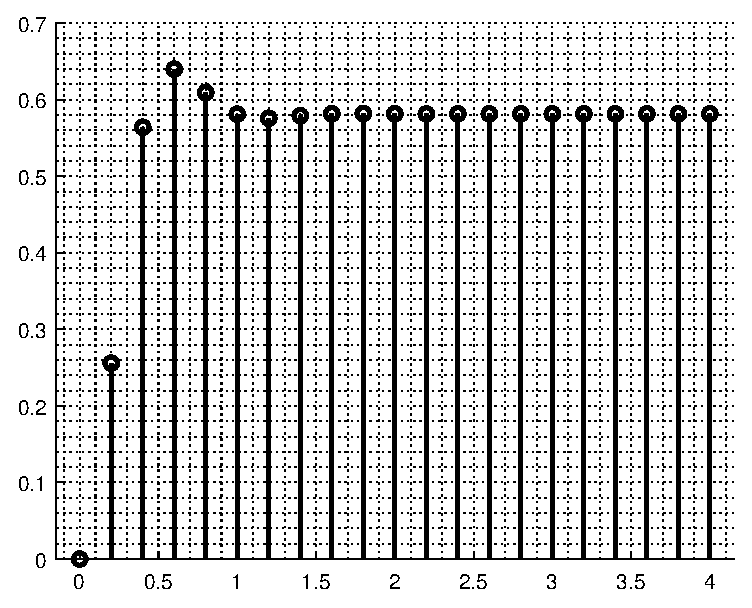
\includegraphics[width=0.75\textwidth]{img/lec8_step1}
    \caption{PD kontrol için kapalı çevrim basamak yanıtı}
    \label{fig:lec8_step1}
\end{figure}
Kapalı çevrim basamak yanıtı isterleri sağlamaktadır, ama giriş işaretini P kontrolör tasarımında olduğu gibi belirli bir hata ile izleyebilmektedir.